%-----------------------------------------------------------------------
% Beginning of chapter.tex
%-----------------------------------------------------------------------
%
%  This is a sample file for use with AMS-LaTeX.  It provides an example
%  of how to set up a file for a book to be typeset with AMS-LaTeX.
%
%  This is the driver file.  Separate chapters should be included at
%  the end of this file.
%
%  ***** DO NOT USE THIS FILE AS A STARTER FOR YOUR BOOK. *****
%  Follow the guidelines in the file chapter.template.
%
%%%%%%%%%%%%%%%%%%%%%%%%%%%%%%%%%%%%%%%%%%%%%%%%%%%%%%%%%%%%%%%%%%%%%%%%

\documentclass[11pt,a4paper]{memoir}
\chapterstyle{demo}
\epigraphfontsize{\small\itshape}
\setlength\epigraphwidth{8cm}
\setlength\epigraphrule{0pt}
\epigraphfontsize{\small\itshape}
%\includeonly{preface,chap1,biblio}

%\numberwithin{section}{chapter}
%\numberwithin{equation}{chapter}

% Include macros here
%=================================================
% Packages
%=================================================

%\usepackage{fixltx2e}
\usepackage[usenames,dvipsnames]{xcolor}
%\usepackage{fancyhdr}
\usepackage{amsmath,amsfonts,amsbsy,amsgen,amscd,mathrsfs,amssymb,amscd}
\usepackage{amsthm}
\usepackage{bm}
\usepackage{url}
\usepackage[UKenglish]{babel}
\usepackage{eurosym}
\usepackage{tikz}
\usepackage{caption}
\usetikzlibrary{matrix,arrows,shapes,calc,3d}
\usepackage{tikz-3dplot}
\tdplotsetmaincoords{60}{110}
\pgfmathsetmacro{\rvec}{.8}
\pgfmathsetmacro{\thetavec}{30}
\pgfmathsetmacro{\phivec}{60}

\tikzset{mynode/.style = {
    % The shape
    circle,
    % The size
    minimum size=2pt,
    % The color
    draw=black, fill=black}
}
\tikzset{vertex/.style={shape=circle, % style for a vertex
                        minimum size=3pt,
                        fill=gray,
                        inner sep = 0pt}}  

% \usepackage{3dplot}
% \tdplotsetmaincoords{60}{110}
%\usepackage{subfig}
\usepackage{microtype}
\usepackage{enumitem}
\usepackage{listings}
\definecolor{darkblue}{rgb}{0,0,.75}

\usepackage[many]{tcolorbox}
\tcbuselibrary{listings}

\definecolor{light-gray}{rgb}{0.96,0.96,0.96}
\definecolor{kwgreen}{rgb}{0,0.5,0}
\definecolor{cogreen}{rgb}{0.25,0.5,0.5}
\definecolor{mygreen}{rgb}{0,0.5,0.125}
\definecolor{equalsign}{rgb}{0.66,0.13,1}
\definecolor{darkred}{rgb}{0.75,0.16,0.37}

\lstloadlanguages{Python} %use listings with Python
%\lstset{literate={==}{{\color{equalsign}==}} {\*}{{\color{equalsign}\*}}}
%\lstnewenvironment{PseudoCode}[1][]
% the space reserved between for the ``In'' numbers and the code
\newlength\inwd
\setlength\inwd{1.7cm}

\newcounter{ipythcntr}

\newtcblisting{ipythonnb}[1][\theipythcntr]{
  enlarge left by=\inwd,
  width=\linewidth-\inwd,
  enhanced,
  boxrule=0.4pt,
  boxsep=0pt,
  left=2pt,
  top=0pt,
  colback=light-gray,
  listing only,
  top=0pt,
  bottom=0pt,
  arc=1pt,
  overlay={
    \node[
      anchor=north east,
      text width=\inwd,
      font=\footnotesize\ttfamily\color{blue!50!black},
      inner ysep=2.5mm,
      inner xsep=0pt,
      outer sep=0pt
      ] 
      at (frame.north west)
      {\stepcounter{ipythcntr}In [#1]:};
  }
  listing style=Python,
  listing options={
    basicstyle=\scriptsize\ttfamily\color{black},
    language=Python,
    escapechar=£,
    showstringspaces=false,
    commentstyle=\color{cogreen},
    keywordstyle=\bfseries\color{kwgreen},
    stringstyle=\color{darkred},
    numberstyle=\color{kwgreen},
    identifierstyle=\color{black},
    %emph={from,import,as},          % Custom highlighting
    otherkeywords={0,1,2,3,4,5,6,7,8,9,\*,==,<=,>=,+,-,\%},
    emph={*,==,<=,>=,+,-,\%},    
    emphstyle=\color{equalsign},
    extendedchars=true,
  },
}

\newtcblisting{ipythonnbout}[1][\theipythcntr]{
  enlarge left by=\inwd,
  width=\linewidth-\inwd,
  enhanced,
  boxrule=0pt,
  boxsep=0pt,
  left=2pt,
  top=0pt,
  colback=white,
  listing only,
  top=0pt,
  bottom=0pt,
  frame hidden,
  overlay={
    \node[
      anchor=north east,
      text width=\inwd,
      font=\footnotesize\ttfamily\color{red},
      inner ysep=2.5mm,
      inner xsep=0pt,
      outer sep=0pt
      ] 
      at (frame.north west)
      {\stepcounter{ipythcntr}Out [#1]:};
  }
  listing style=Python,
  listing options={
    basicstyle=\scriptsize\ttfamily\color{black},
    language=Python,
    escapechar=£,
    showstringspaces=false,
    commentstyle=\color{cogreen},
    keywordstyle=\bfseries\color{kwgreen},
    stringstyle=\color{darkred},
    numberstyle=\color{kwgreen},
    identifierstyle=\color{black},
    %emph={from,import,as},          % Custom highlighting
%    otherkeywords={as,0,1,2,3,4,5,6,7,8,9,\*,==,<=,>=,+,-},
%    emph={*,==,<=,>=,+,-},    
%    emphstyle=\color{equalsign},
    extendedchars=true,
    %literate={#}{{\#}},
  },
}

\newtcblisting{ipythonnboutno}{
  enlarge left by=\inwd,
  width=\linewidth-\inwd,
  enhanced,
  boxrule=0pt,
  boxsep=0pt,
  left=2pt,
  top=0pt,
  colback=white,
  listing only,
  top=0pt,
  bottom=0pt,
  frame hidden,
  overlay={
    \node[
      anchor=north east,
      text width=\inwd,
      font=\footnotesize\ttfamily\color{red},
      inner ysep=2.5mm,
      inner xsep=0pt,
      outer sep=0pt
      ] 
      at (frame.north west)
      {};
  }
  listing style=Python,
  listing options={
    basicstyle=\scriptsize\ttfamily\color{black},
    language=Python,
    escapechar=£,
    showstringspaces=false,
    commentstyle=\color{cogreen},
    %keywordstyle=\bfseries\color{kwgreen},
    stringstyle=\color{darkred},
    numberstyle=\color{kwgreen},
    identifierstyle=\color{black},
    %emph={from,import,as},          % Custom highlighting
    %otherkeywords={as,0,1,2,3,4,5,6,7,8,9,\[,\]},
    %emph={[,]},    
    %emphstyle=\color{black},
    extendedchars=true,
    %literate={#}{{\#}},
  },
}


%{\lstset{language=Matlab,basicstyle=\small, keywordstyle=\color{darkblue},numbers=none,xleftmargin=.04\textwidth,mathescape,frame=single,#1}}
%{}
%\usepackage[]{algorithm2e}
%\usepackage{mcode}
\usepackage{multicol}

%\usepackage[draft]{changes}
%\definechangesauthor[color=blue]{ml}
%\definechangesauthor[color=red]{da}
% \usepackage{trackchanges}
% \addeditor{ml}
% \addeditor{da}

\definecolor{dark-gray}{gray}{0.3}
\definecolor{dkgray}{rgb}{.4,.4,.4}
\definecolor{dkblue}{rgb}{0,0,.5}
\definecolor{medblue}{rgb}{0,0,.75}
\definecolor{rust}{rgb}{0.5,0.1,0.1}

\usepackage[colorlinks=true]{hyperref}
\hypersetup{urlcolor=Blue}
\hypersetup{citecolor=Black}
\hypersetup{linkcolor=dark-gray}

%\usepackage{setspace}
\usepackage{graphicx}
%\usepackage{multicol}
\usepackage{booktabs,longtable,tabu} % Nice tables
\setlength{\tabulinesep}{1pt}
\usepackage{multirow} % More control over tables
\usepackage{float}
\usepackage[T1]{fontenc}
%\usepackage{quotchap}

% Fonts
\usepackage{times}
%\usepackage{fourier}
%\usepackage[no-math]{fontspec}
%\setmainfont{optima}
%\usepackage{charter}
\usepackage{bm} % boldmath must be called after the package

%=================================================
% Paths
%=================================================

\graphicspath{{figures/}}

%=================================================
% Formatting
%=================================================

%\sloppy % Helps with margin justification

%%% Further font changes
\newcommand{\lang}{\textit}
\newcommand{\titl}{\textsl}
\newcommand{\term}{\emph}

%%% Equation numbering
\numberwithin{equation}{section} 

%%% Typesetting
\providecommand{\mathbold}[1]{\bm{#1}}  % Must be after 'fourier'
                                % package loads
%%% Annotations
\newcommand{\notate}[1]{\textcolor{red}{\textbf{[#1]}}}

%=================================================
% Theorem environment
%=================================================

\newtheorem{bigthm}{Theorem}
\renewcommand{\thebigthm}{\Roman{bigthm}}

\newtheorem{theorem}{Theorem}[section]
\newtheorem{lemma}[theorem]{Lemma}
\newtheorem{sublemma}[theorem]{Sublemma}
\newtheorem{proposition}[theorem]{Proposition}
\newtheorem{fact}[theorem]{Fact}
\newtheorem{result}[theorem]{Result}
\newtheorem{conjecture}[theorem]{Conjecture}
\newtheorem{corollary}[theorem]{Corollary}

\newtheorem{problem}[theorem]{Problem}
\newtheorem{solution}[theorem]{Solution}

\theoremstyle{definition}

\newtheorem{definition}[theorem]{Definition}
\newtheorem{example}[theorem]{Example}
\newtheorem{remark}[theorem]{Remark}

\newenvironment{mainthm}{\par\textsc{Main theorem.}\it}{\par}
\renewcommand{\thebigthm}{\Alph{bigthm}}

%=================================================
% Symbols
%=================================================

%%% Old symbols with new names
\newcommand{\oldphi}{\phi}
\renewcommand{\phi}{\varphi}

\newcommand{\eps}{\varepsilon}
\newcommand{\e}{\varepsilon}

%\newcommand{\oldmid}{\mid}
\renewcommand{\mid}{\mathrel{\mathop{:}}} 

%%% New symbols
\newcommand{\defby}{\overset{\mathrm{\scriptscriptstyle{def}}}{=}}
\newcommand{\half}{\tfrac{1}{2}}
\newcommand{\third}{\tfrac{1}{3}}

\newcommand{\sumnl}{\sum\nolimits}

\newcommand{\defeq}{\ensuremath{\mathrel{\mathop{:}}=}} % Definition-equals
\newcommand{\eqdef}{\ensuremath{=\mathrel{\mathop{:}}}} % Equals-definition

%%% Constants
\newcommand{\cnst}[1]{\mathrm{#1}} 
\newcommand{\econst}{\mathrm{e}}
\newcommand{\iunit}{\mathrm{i}}

\newcommand{\onevct}{\mathbf{e}} % All ones vector
\newcommand{\zerovct}{\vct{0}} % Zero vector

\newcommand{\Id}{\mathbf{I}}
\newcommand{\onemtx}{\bm{1}}
\newcommand{\zeromtx}{\bm{0}}

%%% Sets
\newcommand{\coll}[1]{\mathscr{#1}}
\newcommand{\sphere}[1]{S^{#1}}
\newcommand{\ball}[1]{B^{#1}}
\newcommand{\Grass}[2]{\mathbb{G}(#1,#2)}
\providecommand{\mathbbm}{\mathbb} % In case we don't load bbm
\newcommand{\Rplus}{\mathbbm{R}_{+}}
\newcommand{\R}{\mathbbm{R}}
\newcommand{\C}{\mathbbm{C}}
\newcommand{\N}{\mathbbm{N}}
\newcommand{\FF}{\mathbbm{F}}
\newcommand{\struct}{\mathcal{S}}

% Group theory
\newcommand{\stab}{\mathrm{stab}}

% Algebra
\newcommand{\End}{\mathrm{End}}
\newcommand{\Hom}{\mathrm{Hom}}
\newcommand{\Mult}{\mathrm{Mult}}

% Set operations
\newcommand{\polar}{\circ}
\newcommand{\closure}{\overline}
\newcommand{\prtensor}{\,\hat{\otimes}\,}

%%% Real and complex analysis
\newcommand{\abs}[1]{\left\vert {#1} \right\vert}
\newcommand{\abssq}[1]{{\abs{#1}}^2}

\newcommand{\sgn}[1]{\operatorname{sgn}{#1}}
\newcommand{\real}{\operatorname{Re}}
\newcommand{\imag}{\operatorname{Im}}
\newcommand{\pos}{\operatorname{Pos}}
\newcommand{\shrink}{\operatorname{Shrink}}

\newcommand{\diff}[1]{\mathrm{d}{#1}}
\newcommand{\idiff}[1]{\, \diff{#1}}

\newcommand{\gradd}{\mathrm{grad }} % Conflicts w/SIAM styles?
\newcommand{\divv}{\mathrm{div }}
\newcommand{\subdiff}{\partial}

%%% Optimization

\newcommand{\minimize}{\text{minimize}\quad}
\newcommand{\maximize}{\text{maximize}\quad}
\newcommand{\subjto}{\quad\text{subject to}\quad}
\newcommand{\find}{\text{find}\quad}
\newcommand{\suchthat}{\quad\text{such that}\quad}

\newcommand{\argmin}{\operatorname*{arg\; min}}
\newcommand{\argmax}{\operatorname*{arg\; max}}
\newcommand{\dom}{\mathrm{dom} }

%%% Probability & measure

\newcommand{\Prob}{\mathbbm{P}}
\newcommand{\Probe}[1]{\Prob\left({#1}\right)}
\newcommand{\Expect}{\operatorname{\mathbb{E}}}

\newcommand{\St}{\operatorname{St}}

%\newcommand{\normal}{\textsc{Normal}}
\newcommand{\normal}{N}
\newcommand{\uniform}{\textsc{Uniform}}
\newcommand{\erf}{\operatorname{erf}}

\DeclareMathOperator{\rvol}{rvol}
\DeclareMathOperator{\Var}{Var}
\DeclareMathOperator{\Gl}{Gl}
\newcommand{\diag}{\operatorname{diag}}

%%% Vector and matrix operators
\newcommand{\vct}[1]{\mathbold{#1}}
\newcommand{\mtx}[1]{\mathbold{#1}}
\newcommand{\Eye}{\mathbf{I}}

\newcommand{\transp}[1]{#1^{T}}
\newcommand{\trans}{\top}
\newcommand{\adj}{*}
\newcommand{\psinv}{\dagger}

\newcommand{\lspan}[1]{\operatorname{span}{#1}}

\newcommand{\range}{\operatorname{range}}
\newcommand{\colspan}{\operatorname{colspan}}

%\newcommand{\rank}{\operatorname{rank}}
\newcommand{\nullity}{\operatorname{null}}
%\newcommand{\ker}{\operatorname{ker}}
\newcommand{\im}{\operatorname{im}}
%\newcommand{\span}{\operatorname{span}}

%\newcommand{\diag}{\operatorname{diag}}
\newcommand{\trace}{\operatorname{tr}}

\newcommand{\supp}[1]{\operatorname{supp}(#1)}
\newcommand{\sign}[1]{\operatorname{sign}(#1)}

\newcommand{\smax}{\sigma_{\max}}
\newcommand{\smin}{\sigma_{\min}}

\newcommand{\nnz}{\operatorname{nnz}}
\renewcommand{\vec}{\operatorname{vec}}

\newcommand{\Proj}{\ensuremath{\mtx{\Pi}}} % Projection operator

%%% Semidefinite orders
\newcommand{\psdle}{\preccurlyeq}
\newcommand{\psdge}{\succcurlyeq}

\newcommand{\psdlt}{\prec}
\newcommand{\psdgt}{\succ}

%%% Mensuration: inner products and norms

% TeX does not like either \newcommand or \renewcommand for these
% two macros.  There is probably a good reason not to use them via
% \def, but I don't know it.  
%\newcommand{\<}{\langle} 
%\newcommand{\>}{\rangle}
\newcommand{\ip}[2]{\langle {#1}, {#2} \rangle}
% --deleted the \left and \right-- Dennis
% \newcommand{\ip}[2]{\left\langle {#1},\ {#2} \right\rangle}
\newcommand{\absip}[2]{\abs{\ip{#1}{#2}}}
\newcommand{\abssqip}[2]{\abssq{\ip{#1}{#2}}}
\newcommand{\tworealip}[2]{2 \, \real{\ip{#1}{#2}}}

%\newcommand{\norm}[1]{\left\Vert {#1} \right\Vert}
\newcommand{\norm}[1]{\Vert {#1}\Vert}
\newcommand{\normsq}[1]{\norm{#1}^2}

\newcommand{\lone}[1]{\norm{#1}_{\ell_1}}
\newcommand{\smlone}[1]{\|#1\|_{\ell_1}}
\newcommand{\linf}[1]{\norm{#1}_{\ell_\infty}}
\newcommand{\sone}[1]{\norm{#1}_{S_1}}
\newcommand{\snorm}[1]{\sone{#1}}
\newcommand{\wnnorm}[1]{\norm{#1}_{*,\vct{w}}}
\newcommand{\wnnormd}[1]{\norm{#1}^*_{\vct{w}}}
\DeclareMathOperator{\dist}{dist}

% Fixed-size inner products and norms are useful sometimes
\newcommand{\smip}[2]{\bigl\langle {#1}, \ {#2} \bigr\rangle}
\newcommand{\smabsip}[2]{\bigl\vert \smip{#1}{#2} \bigr\vert}
\newcommand{\smnorm}[2]{{\bigl\Vert {#2} \bigr\Vert}_{#1}}

% Specific norms that are used frequently
\newcommand{\enormdangle}{{\ell_2}}
\newcommand{\enorm}[1]{\norm{#1}}
\newcommand{\enormsm}[1]{\enorm{\smash{#1}}}

\newcommand{\enormsq}[1]{\enorm{#1}^2}

\newcommand{\fnorm}[1]{\norm{#1}_{\mathrm{F}}}
\newcommand{\fnormsq}[1]{\fnorm{#1}^2}

\newcommand{\pnorm}[2]{\norm{#2}_{#1}}
%\newcommand{\snorm}[1]{\norm{#1}_*}

\newcommand{\triplenorm}[1]{\left\vert\!\left\vert\!\left\vert {#1} \right\vert\!\right\vert\!\right\vert} 

\newcommand{\flag}[2]{{#1 \brack #2}}

% Special cones
\newcommand{\Feas}{\mathcal{F}}
\newcommand{\Desc}{\mathcal{D}}

\newcommand{\sdim}{\delta}
\newcommand{\sdimw}{\delta^*}
% \newcommand{\sdimw}{\tilde{\delta}}
\newcommand{\ddt}[1]{\dot{#1}}
\DeclareMathOperator{\Circ}{Circ}

%%% Differential geometry
\newcommand{\Cinf}{C^{\infty}}
\newcommand{\Tensf}{\mathcal{T}}
\newcommand{\Vbundle}{\mathcal{X}}
\newcommand{\Christ}[3]{\Gamma_{{#1}{#2}}^{#3}}

% Stuff to be sorted in somewhere
\DeclareMathOperator{\Lip}{Lip}

\newcommand{\IR}{\mathbbm{R}}
\newcommand{\veps}{\varepsilon}
\newcommand{\mA}{\mathcal{A}}
\newcommand{\mB}{\mathcal{B}}
\newcommand{\mC}{\mathcal{C}}
\newcommand{\mD}{\mathcal{D}}
\newcommand{\mE}{\mathcal{E}}
\newcommand{\mI}{\mathcal{I}}
\newcommand{\mM}{\mathcal{M}}
\newcommand{\mN}{\mathcal{N}}
\newcommand{\mL}{\mathcal{L}}
\newcommand{\mV}{\mathcal{V}}
\newcommand{\bface}{\overline{\mathcal{F}}}
\newcommand{\face}{\mathcal{F}}
\newcommand{\relint}{\operatorname{relint}}
\newcommand{\relcl}{\operatorname{relcl}}
\newcommand{\cone}{\operatorname{cone}}
\newcommand{\lin}{\operatorname{lin}}
\newcommand{\Gr}{\operatorname{Gr}}
\newcommand{\powerset}{\mathscr{P}}
\newcommand{\hd}{{\operatorname{hd}}}
\newcommand{\inter}{{\operatorname{int}}}
\newcommand{\conv}{\operatorname{conv}}
\newcommand{\clconv}{\overline{\conv}}
\newcommand{\cl}{\operatorname{cl}}
\newcommand{\bd}{\operatorname{bd}}

\newcommand{\GL}{\operatorname{GL}}

% \newcommand{\tb}{\stackrel{0}{\to}}
\newcommand{\tb}{\,\,\mathring{\to}\,\,}
% \newcommand{\tdash}{\,\,\overset{e}{\to}\,\,}
% \newcommand{\tdash}{\,\,\overset{a}{\to}\,\,}
\newcommand{\tdash}{\overset{a}{\to}}

\newcommand{\K}{\mathcal{K}}
\newcommand{\B}{\mathcal{B}}
\newcommand{\F}{\mathcal{F}}
\newcommand{\D}{\mathcal{D}}
\renewcommand{\P}{\mathcal{P}}
\DeclareMathOperator{\id}{id}
\DeclareMathOperator{\gr}{gr}
\newcommand{\vp}{\varphi}
\newcommand{\maxp}{{\max}_p}
\DeclareMathOperator{\spa}{span}
\DeclareMathOperator{\vol}{vol}
\DeclareMathOperator{\ima}{im}
\DeclareMathOperator{\rk}{rk}

\newcommand{\Ren}{\mathcal{R}}
\newcommand{\T}{\mathcal{T}}
% ADJUST THE FOLLOWING
% \newcommand{\resTMP}[2]{#1,#2}
\newcommand{\resTMP}[2]{#1\to#2}
% 
\newcommand{\res}[3]{\vct{#1}_{\resTMP{#2}{#3}}}
\newcommand{\nres}[3]{\|\vct{#1}\|_{\resTMP{#2}{#3}}}
\newcommand{\sres}[3]{\sigma_{\resTMP{#2}{#3}}(\vct{#1})}
\newcommand{\csres}[3]{\overline{\sigma}_{\resTMP{#2}{#3}}(\vct{#1})}
\newcommand{\kres}[3]{\kappa_{\resTMP{#2}{#3}}(\vct{#1})}
% transpose
\newcommand{\rest}[3]{\vct{#1}^T_{\resTMP{#2}{#3}}}
\newcommand{\nrest}[3]{\|\vct{#1}^T\|_{\resTMP{#2}{#3}}}
\newcommand{\srest}[3]{\sigma_{\resTMP{#2}{#3}}(\vct{#1}^T)}
\newcommand{\csrest}[3]{\overline{\sigma}_{\resTMP{#2}{#3}}(\vct{#1}^T)}
\newcommand{\srestm}[3]{\sigma_{\resTMP{#2}{#3}}(-\vct{#1}^T)}
\newcommand{\krest}[3]{\kappa_{\resTMP{#2}{#3}}(\vct{#1}^T)}
\newcommand{\nresdag}[3]{\|\vct{#1}^\dagger\|_{\resTMP{#2}{#3}}}

\newcommand{\RCD}[3]{\Ren_{#2,#3}(\vct{#1})}
% \newcommand{\RCD}[3]{\Ren_{\resTMP{#2}{#3}}(\vct{#1})}

\newcommand{\DA}{\vct{\Delta A}}

%
\newcommand{\Rmm}{R_{\mathrm{mm}}}

\newcommand{\rbinom}[2]{\genfrac{[}{]}{0pt}{}{#1}{#2}}
\newcommand{\trbinom}[2]{{\textstyle\genfrac{[}{]}{0pt}{}{#1}{#2}}}

\newcommand{\comm}[1]{\textcolor{red}{\textbf{[#1]}}}
\newcommand{\rant}[1]{\textcolor{blue}{\textbf{[#1]}}}
%

\newcommand{\llangle}{\langle\hspace{-1.5pt}\langle}  % this is actually contained in mnsymbol, but loading this package causes trouble...
\newcommand{\rrangle}{\rangle\hspace{-1.5pt}\rangle}  % this is actually contained in mnsymbol, but loading this package causes trouble...

\newcommand{\Res}{\mathrm{Res}}
\newcommand{\Oh}{\mathcal{O}}
\newcommand{\Mbar}{\overline{M}}
\newcommand{\second}{\mathrm{II}}
\newcommand{\nablabar}{\overline{\nabla}}
\newcommand{\expm}{\mathrm{exp}}
\newcommand{\Rc}{\mathrm{Rc}}
\newcommand{\NJ}{\mathrm{NJ}}
% %\newcommand{\GL}[1]{\mathrm{GL}(#1)}

\newcommand{\cover}{\lessdot}

% Semidefinite programming
\newcommand{\Sym}{\mathcal{S}}
\newcommand{\SDP}{\mathcal{S}_+}
\newcommand{\psd}{\succeq}
\newcommand{\bdot}{\bullet}

%\renewcommand{\chaptername}{}
%\renewcommand{\thechapter}{}

\begin{document}
\numberwithin{section}{chapter}
\numberwithin{equation}{chapter}
\numberwithin{theorem}{chapter}

\lstset{language=Matlab}

%\frontmatter
%\title{Convex Optimization}

%    Information for first author
%\author{Martin Lotz}
%    Address of record for the research reported here

%\address{School of Mathematics\\ The University of Manchester\\ Alan Turing Building, Oxford Road\\ Manchester M139PL}

%\email{martin.lotz@manchester.ed.uk}
%\urladdr{http://www.maths.manchester.ac.uk/\textasciitilde mlotz}

%\date{\today}

%\maketitle

%\newpage 

%\tableofcontents

%\include{preface}

\mainmatter

%\include{notation}
%-----------------------------------------------------------------------
% Beginning of chap1.tex
%-----------------------------------------------------------------------
%
%  AMS-LaTeX sample file for a chapter of a monograph, to be used with
%  an AMS monograph document class.  This is a data file input by
%  chapter.tex.
%
%  Use this file as a model for a chapter; DO NOT START BY removing its
%  contents and filling in your own text.
% 
%%%%%%%%%%%%%%%%%%%%%%%%%%%%%%%%%%%%%%%%%%%%%%%%%%%%%%%%%%%%%%%%%%%%%%%%


\chapter*{Lecture 1}
\addcontentsline{toc}{chapter}{Lecture 1}
\addtocounter{chapter}{1}
%\numberwithin{section}{chapter}
\numberwithin{equation}{chapter}
\numberwithin{theorem}{chapter}

\epigraph{``[N]othing at all takes place in the universe in which some rule of maximum or minimum does not appear.''}{--- \textup{Leonhard Euler}}

Mathematical optimization, traditionally also known as mathematical programming, is the theory of optimal decision making. Optimization problems arise in a large variety of contexts, including scheduling and logistics problems, finance, optimal control, signal processing, and machine learning. The underlying mathematical problem always amounts to finding parameters that minimize\footnote{For the sake of consistency with most of the literature, throughout these notes we use the American spelling of minimizer and maximizer with ``z'' instead of ``s''.} (cost) or maximize (utility) an objective function in the presence or absence of a set of constraints. An important special case is the class of {\em convex optimization} problems. Such problems will be the main focus of this course.

\section{What is an optimization problem?}
A general mathematical optimization problem is a problem of the form
\begin{align}\label{eq:opt-form}
\begin{split}
 \minimize & f(\vct{x})\\
 \subjto & \vct{x}\in \Omega
 \end{split}
\end{align}

where $f\colon \R^n\to \R$ are real-valued \textbf{objective function} and $\Omega\subseteq \R^n$ is a set defining the \textbf{constraints}.
Among all $\vct{x}\in \Omega$, we seek one with smallest $f$-value. Typically, the constraint set $\Omega$ will consist of such $\vct{x}\in \R^n$ that satisfy certain equations and inequalities,

\begin{equation*}
f_1(\vct{x})\leq 0, \dots, f_m(\vct{x})\leq 0, g_1(\vct{x})=0, \dots, g_p(\vct{x})=0.
\end{equation*}

A vector $\vct{x}^*$ satisfying the constraints is called an {\em optimum}, a {\em solution}, or a {\em minimizer} of the problem~\eqref{eq:opt-form}, if $f(\vct{x}^*)\leq f(\vct{x})$ for all other $\vct{x}$ that satisfy the constraints. Note that replacing $f$ by $-f$, we could equivalently state the problem as a maximization problem. In this course we are mostly concerned with functions and constraint sets that are \textbf{convex}.

\begin{itemize}
\item A set $C\subseteq \R^n$ is \textbf{convex}, if for all $\vct{x},\vct{y}\in C$ and $\lambda\in [0,1]$, $\lambda \vct{x}+(1-\lambda)\vct{y}\in C$. That is, for any two points in $C$, the line segment connecting them is also in $C$. 
\item A function $f\colon C\to \R$ is convex, if $C$ is convex and for all $\vct{x}, \vct{y}\in C$ and $\lambda\in [0,1]$, $f(\lambda \vct{x}+(1-\lambda)\vct{y})\leq \lambda f(\vct{x})+(1-\lambda)f(\vct{y})$. 
\end{itemize}

\begin{figure}
\centering
\begin{minipage}{0.45\textwidth}
\begin{tikzpicture}[thick,rotate=15,scale=0.8]
\filldraw[color=black, fill=blue!5, very thick, rotate=15](0,0) ellipse (2 and 1.2);

\node (A1) at (-1,0)  [label=180:${\textbf{x}}$] {};
\node (A2) at (1,0)   [label=0:${\textbf{y}}$] {};
\filldraw[black] (-0.9,0) circle (2pt);
\filldraw[black] (0.9,0) circle (2pt);

\draw[color=blue,thick] (A1) -- (A2);
\end{tikzpicture}
\end{minipage}
%
\begin{minipage}{0.45\textwidth}
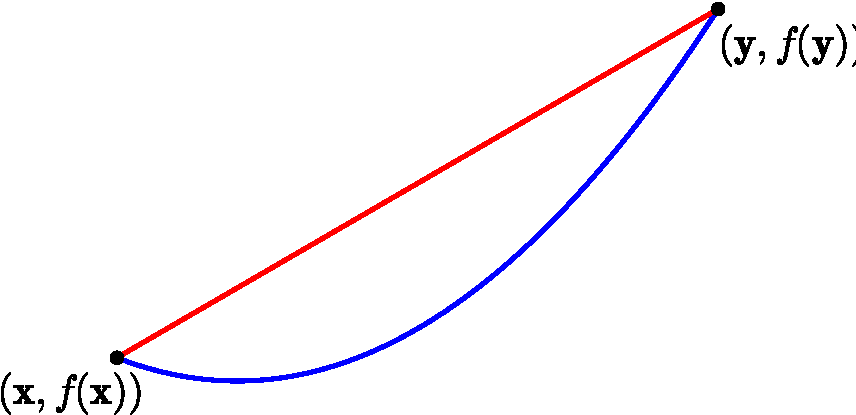
\includegraphics[width=1.0\textwidth]{images/convf-crop.pdf}
\end{minipage}
\caption{A convex set and a convex function}
\end{figure}

A \textbf{convex optimization} problem is one where the set of constraints $\Omega$ and the function $f$ are convex. While most general optimization problems are practically intractable, convex optimization problems can be solved efficiently, and still cover a surprisingly large range of applications!

\section{Examples of optimization problem}
Countless problems from science and engineering can be cast as optimization problems. We present a few first examples, many more will follow in the course of this lecture. The examples below come with associated Python code. At this moment it is not expected that you understand them in detail, they are merely intended to illustrate some of the problems that convex optimization deals with, and how they can be solved.

\begin{example}\label{ex:1}
Suppose we want to understand the relationship of a quantity $Y$ (for example, sales data) to a series of {\em predictors} $X_1,\dots,X_p$ (for example, advertising budget in different media). We can often assume the relationship to be {\em approximately linear},

\addtocounter{equation}{1}
\begin{equation}\label{eq:linreg1}
 Y = \beta_0+\beta_1 X_1 + \cdots + \beta_p X_p + \varepsilon, 
\end{equation}
where $\varepsilon$ is some error or noise term. The goal is to determine the {\em model parameters} $\beta_0,\dots,\beta_p$.
To determine these, we can collect $n\geq p$ sample realizations (from observations or experiments),

\begin{equation*}
 Y=y_i, \quad X_1=x_{i1},\dots,X_p=x_{ip}, \quad 1\leq i\leq n,
\end{equation*}

and assume that the data is related according to~\eqref{eq:linreg1}, 

\begin{equation*}
 y_i = \beta_0+\beta_1x_{i1}+\cdots +\beta_p x_{ip}+\varepsilon_i, \quad 1\leq i\leq n.
\end{equation*}

Collecting the data in matrices and vectors,

\begin{equation*}
 \vct{y} = \begin{pmatrix}
            y_1\\ \vdots \\ y_n
           \end{pmatrix},
\quad \mtx{X} = \begin{pmatrix} 
           1 & x_{11} & \cdots & x_{1p}\\
           \vdots & \vdots & \ddots & \vdots \\
           1 & x_{n1} & \cdots & x_{np}
          \end{pmatrix},
\quad \vct{\beta} = \begin{pmatrix}
                     \beta_0\\
                     \beta_1\\
                     \vdots\\
                     \beta_p
                    \end{pmatrix},
\quad \vct{\varepsilon} = \begin{pmatrix}
                  \e_1\\
                  \vdots\\
                  \e_n
                 \end{pmatrix},
\end{equation*}

we can write the relationship concisely as 

\begin{equation*}
 \vct{y} = \mtx{X}\vct{\beta}+\vct{\e}.
\end{equation*}

We would then like to find $\vct{\beta}$ in such a way that the difference $\vct{\e}=\vct{y}-\mtx{X}\vct{\beta}$ is as {\em small} as possible. One way of measuring the size of a vector $\vct{x}\in \R^n$ is the square of its $2$-norm, or Euclidean norm, 

\begin{equation*}
 \norm{\vct{x}}_2^2=\vct{x}^{\trans}\vct{x}=\sum_{i=1}^nx_i^2.
\end{equation*}

The best $\vct{\beta}$ is then the vector that solves the unconstrained optimization problem

\begin{equation*}
 \minimize \norm{\mtx{X}\vct{\beta}-\vct{y}}_2^2.
\end{equation*}

This is an example of an optimization problem, with variables $\vct{\beta}$, no constraints ({\em all} $\beta$ are valid candidates and the constraint set is $\Omega=\R^{p+1}$), and a {\em quadratic} objective function 

\begin{equation*}
f(\vct{\beta})=\norm{\mtx{X}\vct{\beta}-\vct{y}}_2^2 = (\mtx{X}\vct{\beta}-\vct{y})^{\trans}(\mtx{X}\vct{\beta}-\vct{y}) = \vct{\beta}^{\trans}\mtx{X}^{\trans}\mtx{X}\vct{\beta}-2\vct{y}^{\trans}\mtx{X}\vct{\beta}+\vct{y}^{\trans}\vct{y},
\end{equation*}

where $\mtx{X}^{\trans}$ is the matrix transpose.
As we will see later, quadratic functions are convex, so this is a convex optimization problem.
This simple optimization problem has a **unique closed form solution**,

\begin{equation}\label{eq:least1}
 \vct{\beta}^* = (\vct{X}^{\trans}\vct{X})^{-1}\vct{X}^{\trans}\vct{y}.
\end{equation}

In practice one wouldn't compute $\vct{\beta}^*$ by evaluating [1], as there are more efficient methods available (see Lecture 2). 
%Suppose we want to understand the relationship of a quantity $Y$ (for example, sales data) to a series of {\em predictors} $X_1,\dots,X_n$ (for example, advertising budget in different media). In many situations there is reason to assume that the relationship as approximately linear,
% \begin{equation}\label{eq:linreg1}
%  Y = \beta_0+\beta_1X_1+\cdots+\beta_p X_p+\e,
% \end{equation}
%where $\e$ is some random error. The goal is to determine the {\em model parameters} $\beta_0,\dots,\beta_p$.
%To determine these, we can collect $n\geq p$ sample realizations (from observations or experiments),
%\begin{equation*}
% Y=y_i, \quad X_1=x_{i1},\dots,X_p=x_{ip}, \quad 1\leq i\leq n,
%\end{equation*}
%and assume that the data is related according to~\eqref{eq:linreg1}, 
%\begin{equation*}
% y_i = \beta_0+\beta_1x_{i1}+\cdots +\beta_p x_{ip}+\e_i, \quad 1\leq i\leq n.
%\end{equation*}
%Collecting the data in matrices and vectors,
%\begin{equation*}
% \vct{y} = \begin{pmatrix}
%            y_1\\ \vdots \\ y_n
%           \end{pmatrix},
%\quad \mtx{X} = \begin{pmatrix} 
%           1 & x_{11} & \cdots & x_{1p}\\
%           \vdots & \ddots & \vdots \\
%           1 & x_{n1} & \cdots & x_{np}
%          \end{pmatrix},
%\quad \vct{\beta} = \begin{pmatrix}
%                     \beta_0\\
%                     \beta_1\\
%                     \vdots\\
%                     \beta_p
%                    \end{pmatrix},
%\quad \vct{\e} = \begin{pmatrix}
%                  \e_1\\
%                  \vdots\\
%                  \e_n
%                 \end{pmatrix},
%\end{equation*}
%we can write the relationship concisely as 
%\begin{equation*}
% \vct{y} = \mtx{X}\vct{\beta}+\vct{\e}.
%\end{equation*}
%We would then like to find $\vct{\beta}$ in such a way that the difference $\vct{\e}=\vct{y}-\mtx{X}\vct{\beta}$ is as ``small'' as possible. A standard way of measuring the size of a vector is the square of its {\em 2-norm}, or Euclidean norm, 
%\begin{equation*}
% \norm{\vct{x}}_2^2=\vct{x}^{\trans}\vct{x}=\sum_{i=1}^dx_i^2.
%\end{equation*}
%The best $\vct{\beta}$ is then the vector that solves the unconstrained optimization problem
%\begin{equation*}
% \minimize \norm{\mtx{X}\vct{\beta}-\vct{y}}_2^2.
%\end{equation*}
%This is an optimization problem of the form~\eqref{eq:opt-form}, with variables $\vct{\beta}$, $m=0$ constraints, and a {\em quadratic} objective function $f(\vct{\beta})=\norm{\mtx{X}\vct{\beta}-\vct{y}}_2^2$.
%This simple optimization problem has a {\em unique closed form solution},
%\begin{equation}\label{eq:least1}
% \vct{\beta}^* = (\vct{X}^{\trans}\vct{X})^{-1}\vct{X}^{\trans}\vct{y},
%\end{equation}
%where $\vct{X}^{\trans}$ is the matrix transpose. In practice one wouldn't compute $\vct{\beta}^*$ by evaluating ~\eqref{eq:least1}, as there are more efficient methods available (see Lecture 2).

To illustrate the least squares setting using a concrete example, assume that we have data relating the basal metabolic rate (energy expenditure per time unit) in mammals to their mass.\footnote{This example is from the episode ``Size Matters'' of the BBC series Wonders of Life.}
\begin{figure}[h!]
\centering
 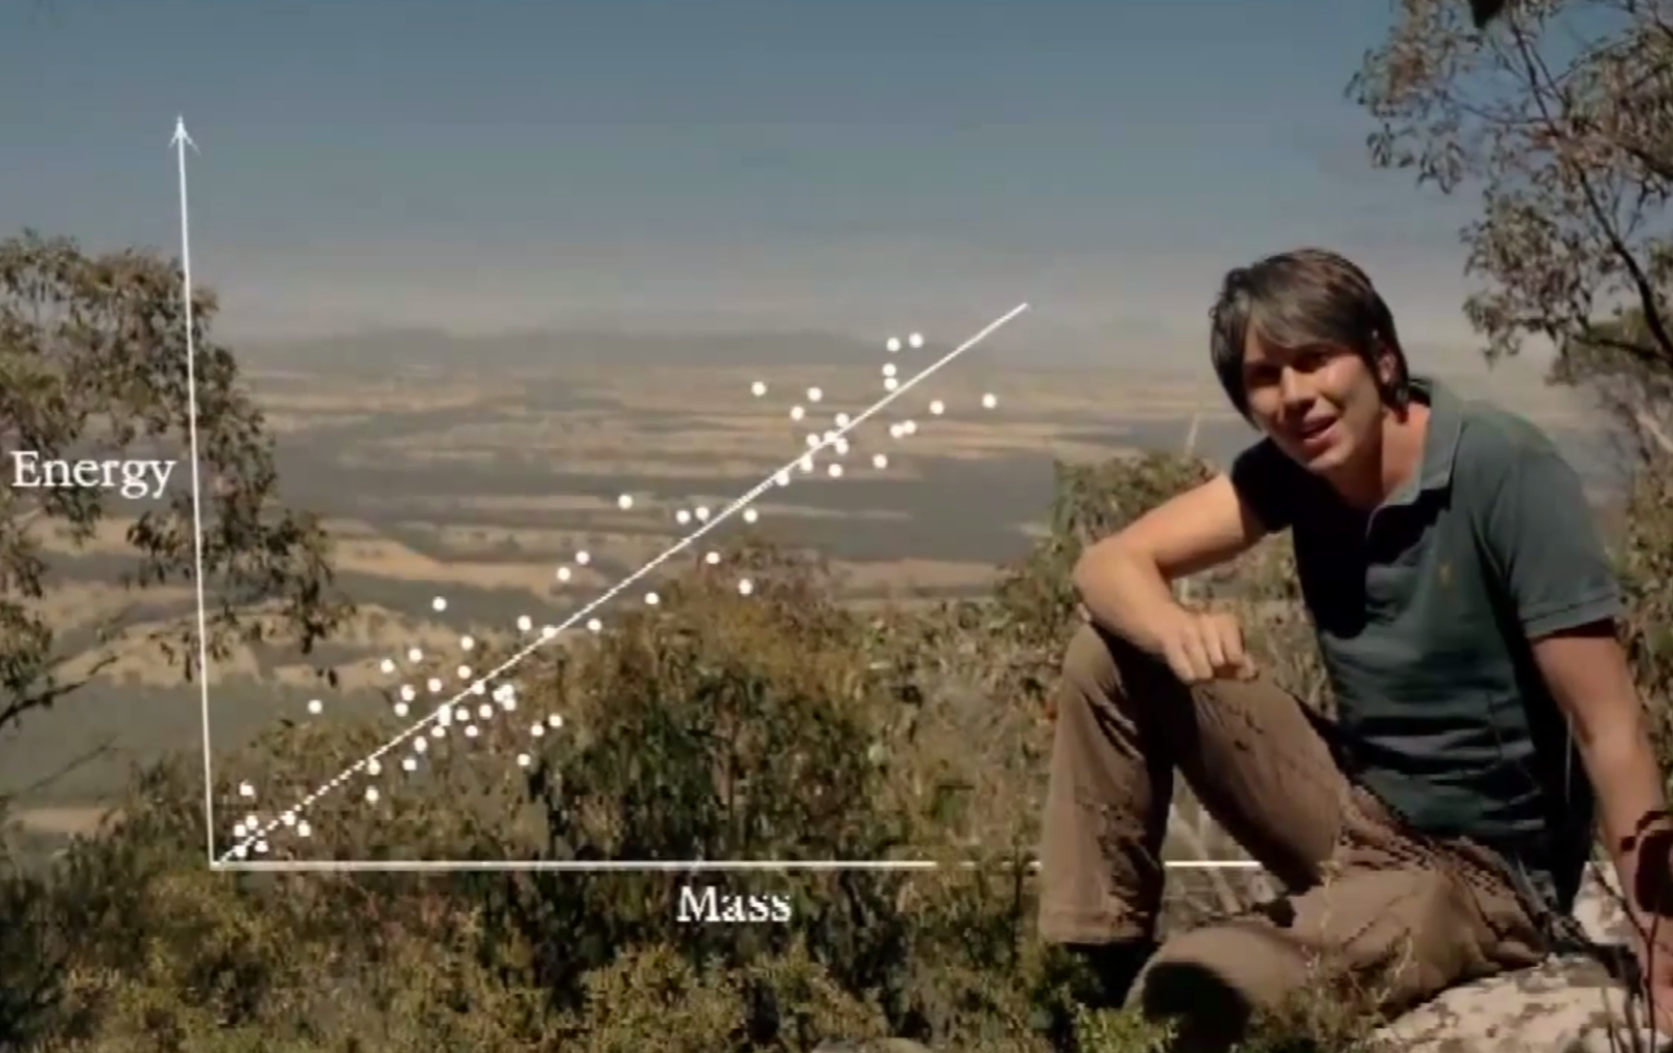
\includegraphics[width=0.6\textwidth]{images/briancox.png}
\end{figure}
The model we use is $Y=\beta_0+\beta_1X$, with $Y$ the basal metabolic rate and $X$ the mass. Using data for 573 mammals from the PanTHERIA database\footnote{\url{http://esapubs.org/archive/ecol/E090/184/\#data}}, we can assemble the vector $\vct{y}$ and the matrix $\mtx{X}\in \R^{n\times (p+1)}$ in order to compute the $\vct{\beta}=(\beta_0,\beta_1)^{\trans}$. Here, $p=1$ and $n=573$.

We next illustrate how to solve this problem in Python. As usual, we first have to import some relevant libraries: \textbf{numpy} for numerical computation, \textbf{pandas} for loading and transforming datasets, \textbf{cvxpy} for convex optimization, and \textbf{matplotlib} for plotting.

\begin{ipythonnb}
\\# Import some important Python modules
import numpy £\bfseries\color{kwgreen}as£ np
import pandas £\bfseries\color{kwgreen}as£ pd
from cvxpy import *
import matplotlib.pyplot as plt
\end{ipythonnb}

We next have to load the data. The data is saved in a table with 573 rows and 2 columns, where the first column list the mass and the second the basal metabolic rate.

\begin{ipythonnb}
\\# Load data into numpy array
bmr = pd.read_csv('../../data/bmr.csv',header=None).as_matrix()
# We can find out the dimension of the data
bmr.shape
\end{ipythonnb}
\begin{ipythonnbout}[2]
(573, 2)
\end{ipythonnbout}

To see the first three and the last three rows of the dataset, we can use the "print" command.

\begin{ipythonnb}[3]
print(bmr[0:3,:])
\end{ipythonnb}

\begin{ipythonnboutno}
[[ 13.108   10.604 ]
 [  9.3918   8.2158]
 [ 10.366    9.3285]]
\end{ipythonnboutno}

To visualise the whole dataset, we can make a scatterplot by interpreting each row as a coordinate on the plane, and marking it with a dot.

\begin{ipythonnb}[4]
# Display scatterplot of data (plot all the rows as points)
% matplotlib inline
bmr£1£ = plt.plot(bmr[:,0],bmr[:,1],'o')
plt.xlabel("Mass")
plt.ylabel("Basal metabolic rate")
plt.show()
\end{ipythonnb}

\begin{figure}[h!]
\centering
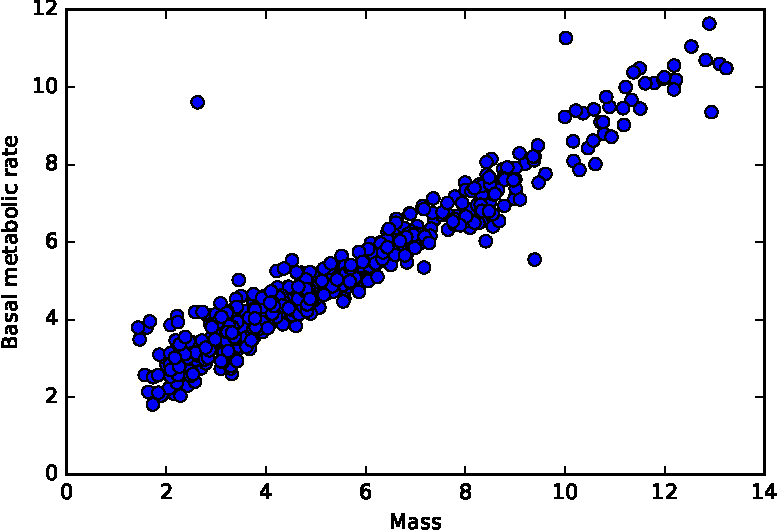
\includegraphics[width=0.9\textwidth]{images/bmr1-crop.pdf}
\end{figure}

The plot above suggests that the relation of the basal metabolic rate to the mass is linear, i.e., of the form
\begin{equation*}
  Y = \beta_0+\beta_1 X,
\end{equation*}
where X is the mass and Y the BMR. We can find $\beta_0$ and $\beta_1$ by solving an optimization problem as described above. We first have to assemble the matrix $\mtx{X}$ and the vector $\vct{y}$.

\begin{ipythonnb}[5]
n = bmr.shape[0]
p = 1
X = np.concatenate((np.ones((n,1)),bmr[:,0:p]),axis=1)
y = bmr[:,-1]
\end{ipythonnb}

\begin{ipythonnb}[6]
# Create a (p+1) vector of variables
Beta = Variable(p+1)

# Create sum-of-squares objective function
objective = Minimize(sum_entries(square(X*Beta - y)))

# Create problem and solve it
prob = Problem(objective)
prob.solve()

print("status: ", prob.status)
print("optimal value: ", prob.value)
print("optimal variables: ", Beta[0].value, Beta[1].value)
\end{ipythonnb}
\begin{ipythonnboutno}
status:  optimal
optimal value:  152.736200529558
optimal variables:  1.3620698558275837 0.7016170245505547
\end{ipythonnboutno}

Now that we solved the problem and have the values $\beta_0 = 1.362$ and $\beta_1 = 0.702$, we can plot the line and see how it fits the data.

\begin{ipythonnb}[6]
plt.plot(bmr[:,0],bmr[:,1],'o')

xx = np.linspace(0,14,100)
bmr = plt.plot(xx, Beta[0].value+Beta[1].value*xx, color='red',\
 linewidth=2)
plt.show()
\end{ipythonnb}

\begin{figure}[h!]
\centering
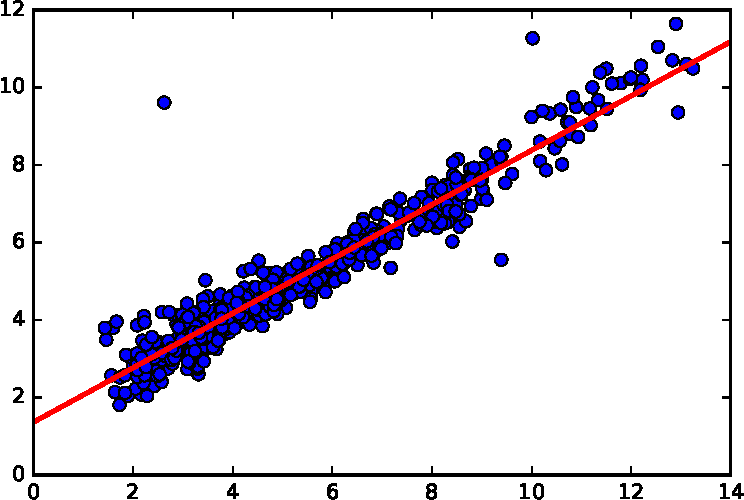
\includegraphics[width=0.9\textwidth]{images/bmr2-crop.pdf}
\end{figure}

Even though for illustration purposes we used the CVXPY package, this particular problem can be solved directly using the least squares solver in numpy.

\begin{ipythonnb}[7]
import numpy.linalg £\bfseries\color{kwgreen}as£ la
beta = la.lstsq(X,y)
print(beta[0])
\end{ipythonnb}
\begin{ipythonnboutno}
[ 1.36206997  0.70161692]
\end{ipythonnboutno}
\end{example}

The above example is an example of a \textbf{machine learning} problem. In machine learning, one seeks to {\em learn} a function $F$ mapping some inputs $X$ to outputs $Y$, $Y=F(X)$. A few examples:
\begin{itemize}
\item $X$: economic data, $Y$: value of a stock;
\item $X$: physiological data, $Y$: medical diagnosis;
\item $X$: email, $Y$: $1$ if email is span, $0$ otherwise;
\item $X$: scanned image, $Y$: a letter represented by that image.
\end{itemize}

In {\em supervised learning} we have a set of sample input pairs, $(y_i,x_i)$, $1\leq i\leq m$, and we typically try to find a function $F$ that minimizes the \textbf{least squared error},

\begin{equation*}
  \minimize \sum_{i=1}^m (\vct{y}_i-F(\vct{x}_i))^2,
\end{equation*}

where one minimizes over all functions $F$ from some class. In the above example, we assumed our functions to be linear, in which case the can by parametrized by the coefficients $\beta_0, \dots,\beta_p$. As the course progresses, we will see examples of more sophisticated machine learning problems, often with nonlinear objective function and other {\em loss functions} instead of the least square error. 

\begin{example}\label{ex:2}(Linear programming)
 Suppose a plane has two cargo compartments with weight capacities $C_1=35$ and $C_2=40$ tonnes, and volumes (space capacities) $V_1=250$ and $V_2=400$ cubic metres. Assume we have three types of cargo to transport, specified as follows.
 
 \begin{figure}[h!]
 \begin{tabular}{r | c | c | c}
           & Volume (m$^3$ per tonne) & Weight (tonnes) & Profit (\pounds / tonne)\\
           \hline 
   Cargo 1 &  8    &  25 & \pounds 300\\
   \hline 
   Cargo 2 &  10    &  32 & \pounds 350\\
   \hline
   Cargo 3 & 7    & 28  & \pounds 270\\
   \hline
 \end{tabular}
 \end{figure}

 The problem is now to decide how much of each cargo to take on board, and how to distribute it in an optimal way among the two compartments.
 \begin{enumerate}
  \item The {\em decision variables} $x_{ij}$ specify the amount, in tonnes, of cargo $i$ to go into compartment $j$. We collect them in a vector $\vct{x}$.
  \item The {\em objective function} is the total profit, 
  \begin{equation*}
   f(\vct{x}) = 300\cdot (x_{11}+x_{12})+ 350\cdot (x_{21}+x_{22})+270\cdot (x_{31}+x_{32}).
  \end{equation*}
\item The {\em constraints} are given by the space and weight limitations of the compartments, and the amount of cargo available.
{\small
\begin{align*}
 x_{11}+x_{12} & \leq 25 \quad \text{ (total amount of cargo 1)}\\ 
 x_{21}+x_{22} & \leq 32 \quad \text{ (total amount of cargo 2)}\\ 
 x_{31}+x_{32} & \leq 28 \quad \text{ (total amount of cargo 3)}\\
 x_{11}+x_{21}+x_{31} & \leq 35 \quad \text{ (weight constraint on compartment 1)}\\
 x_{12}+x_{22}+x_{32} & \leq 40 \quad \text{ (weight constraint on compartment 2)}\\
 8x_{11}+10x_{21}+7x_{31} & \leq 250 \quad \text{ (volume constraint on compartment 1)}\\
 8x_{12}+10x_{22}+7x_{32} & \leq 400 \quad \text{ (volume constraint on compartment 2)}\\
 (x_{11}+x_{21}+x_{31})/35 - (x_{12}+x_{22}+x_{32})/40 &= 0 \quad \text{ (maintain balance of weight ratio)}\\
 x_{ij} &\geq 0 \quad \text{ (cargo can't have negative weight)}
\end{align*}}
 \end{enumerate}

 It is customary to write the objective function as a scalar product, $f(\vct{x}) = \ip{\vct{c}}{\vct{x}} := \vct{c}^{\trans}\vct{x}$, and to express the constraints as systems of linear equations and inequalities using matrix-vector products,
 \begin{align*}
  \maximize &\ip{\vct{c}}{\vct{x}} \\
  \subjto &A\vct{x}\leq \vct{b}\\
  & B\vct{x} = \vct{d}\\
          & \vct{x}\geq 0        
 \end{align*}
where the inequalities $\geq$ and $\leq$ are to be understood componentwise.
 This problem has a unique solution that can be found using CVXPY in Python,
 
\begin{ipythonnb}[8]
\\# Define all the matrices and vectors involved
c = np.array([300,300,350,350,270,270])
A = np.array([[1, 1, 0, 0, 0, 0],
              [0, 0, 1, 1, 0, 0],
              [0, 0, 0, 0, 1, 1],
              [1, 0, 1, 0, 1, 0],
              [0, 1, 0, 1, 0, 1],
              [8, 0, 10, 0, 7, 0],
              [0, 8, 0, 10, 0, 7]])
b = np.array([25,32,28,35,40,250,400]);
B = np.array([1/35, -1/40, 1/35, -1/40, 1/35, -1/40]);
d = np.zeros(1)

# Create variables, objective and constraints
x = Variable(6)
constraints = [A*x <= b, B*x == d, x >= 0]
objective = Maximize(c*x)

# Create a problem using the objective and constraints and solve it
prob = Problem(objective, constraints)
prob.solve()

print("Solution found: \n", np.round(np.abs(x.value), \
  decimals=2).transpose())
\end{ipythonnb}
\begin{ipythonnboutno}
Solution found: 
 [[  6.75   7.71   0.    32.    28.     0.  ]]
\end{ipythonnboutno}

The solution found is
 \begin{equation*}
 x_{11} = 6.7500 , x_{12} =  7.7143, x_{21} = 0, x_{22} = 32, x_{31} = 28, x_{32} = 0.
 \end{equation*}

 We made some simplifying assumptions, for example that the cargo can be split up into arbitrary fractions. Additional work is required to resolve these issues.
 Problems of this kind are known as \textbf{linear programming}, because the objective function and the constraints are given by linear functions. Such problems can be solved efficiently using the simplex algorithm or interior point methods. The highly developed theory of linear programming acts as a template for more general convex optimization that is developed in this course.
\end{example}
%
%\begin{example}(Portfolio optimization)
%Suppose we would like to invest a certain amount of money among $n$ assets (for example, stocks), with $x_i$ denoting the proportion that we put in asset $i$. The {\em return} of asset prices is the relative change in price from one period to the next,
%\begin{equation*}
% r = \frac{p_{\text{new}}-p_{\text{old}}}{p_{\text{old}}},
%\end{equation*}
%where $p_{\text{new}}$ and $p_{\text{old}}$ denote the old an new prices. If asset $i$ has return $r_i$, then the return of the whole portfolio is $r = x_1r_1+\cdots +x_nr_n$.
%As we do not know the true future returns $r_i$, we have to work with statistical estimates $\mu_i$ (for example, the sample mean of previous data). The total expected return of the portfolio is then
%\begin{equation*}
% \mu = x_1\mu_1+\cdots x_n\mu_n = \vct{\mu}^{\trans}\vct{x},
%\end{equation*}
%where $\vct{\mu}=(\mu_1,\dots,\mu_n)^{\trans}$ and $\vct{x}=(x_1,\dots,x_n)^{\trans}$.
%
%The goal is to select the proportions $\vct{x}$ in order to achieve a target expected return, while keeping the {\em risk} as small as possible. The risk can be measured in various ways, one being through a {\em correlation matrix} $\mtx{\Sigma}$ estimated from factors and past data. The risk of taking the positions $\vct{x}$ can then be modelled as the quadratic function $\vct{x}^{\trans}\mtx{\Sigma}\vct{x}$. The optimization problem we arrive at is
%\begin{align*}
% \minimize & \vct{x}^{\trans}\mtx{\Sigma}\vct{x}\\
% \subjto & \vct{\mu}^{\trans}\vct{x} = \mu\\
% & \sum_{i=1}^n x_i=1\\
% & \vct{x}\geq 0.
%\end{align*}
%Like Example~\ref{ex:1}, this problem involves minimizing a quadratic function, and like Example~\ref{ex:2}, it has linear equalities and inequalities as constraints. If we take away the inequality $\vct{x}\geq 0$ (in financial terms, this corresponds to allowing short-selling), then we can get a closed form solution using the method of Lagrange multipliers.
%\end{example}

\begin{example}(Image inpainting)
Optimization methods play an increasingly important role in image and signal processing. An image can be viewed as an $m\times n$ matrix $\mtx{U}$, with each entry $u_{ij}$ corresponding to a light intensity (for greyscale images), or a colour vector, represented by a triple of red, green and blue intensities (usually with values between $0$ and $255$ each). For simplicity the following discussion assumes a greyscale image. For compututational pursposes, the matrix of an image is often viewed as an $mn$-dimensional vector $\vct{u}$, with the columns of the matrix stacked on top of each other. 

In the {\em image inpainting} problem, one aims to {\em guess} the true value of missing or corrupted entries of an image. There are different approaches to this problem. A conceptually simple approach is to replace the image with the {\em closest} image among a set of images satisfying typical properties. But what are typical properties of a typical image? Some properties that come to mind are:

\begin{itemize}
\item Images tend to have large homogeneous areas in which the colour doesn't change much;
\item Images have approximately low rank, when interpreted as matrices.
\end{itemize}

Total variation image analysis takes advantage of the first property. The \textbf{total variation} or TV-norm is the sum of the norm of the horizontal and vertical differences,

\begin{equation*}
  \|\vct{U}\|_{\mathrm{TV}} = \sum_{i=1}^m \sum_{j=1}^n \sqrt{(u_{i+1,j}-u_{i,j})^2+(u_{i,j+1}-u_{i,j})^2},
\end{equation*}

where we set entries with out-of-bounds indices to $0$. The TV-norm naturally increases with increased variation or sharp edges in an image. Consider for example the two following matrices (imagine that they represent a $3\times 3$ pixel block taken from an image).

\begin{equation*}
\mtx{U}_1 = \begin{pmatrix}
 0 & 17 & 3 \\
 7 & 32 & 0 \\
 2 & 9 & 27
\end{pmatrix}, \quad
\mtx{U}_2\begin{pmatrix}
1 & 1 & 3\\
1 & 0 & 0\\
0 & 0 & 2
\end{pmatrix}
\end{equation*}

The left matrix has TV-norm $\|\mtx{U}_1\|_{\mathrm{TV}} = 200.637$, while the right one has TV-norm $\|\mtx{U}_2\|_{\mathrm{TV}} = 14.721$ (verify this!) Intuitively, we would expect a natural image with artifacts added to it to have a higher TV norm.

Now let $\mtx{U}$ be an image with entries $u_{ij}$, and let $\Omega\subset [m]\times [n] = \{(i,j) \mid 1\leq i\leq m, 1\leq j\leq n\}$ be the set of indices where the original image and the corrupted image coincide (all the other entries are missing). One could attempt to find the image with the {\em smallest} TV-norm that coincides with the knwon pixels $u_{ij}$ for $(i,j)\in \Omega$. This is an optimization problem of the form

\begin{equation*}
  \minimize \|\vct{X}\|_{\mathrm{TV}} \subjto x_{ij} = u_{ij} \text{ for } (i,j) \in \Omega.
\end{equation*}

The TV-norm is an example of a convex function and the constraints are linear conditions which define a convex set. This is again an example of a \textbf{convex optimization problem} and can be solved efficiently by a range of algorithms. For the time being we will not go into the algorithms but solve it using CVXPY. The example below is based on an example from the CVXPY Tutorial\footnote{\url{http://www.cvxpy.org/en/latest/tutorial/index.html}}, and it is recommended to look at this tutorial for other interesting examples! 

\textbf{Warning}: the example below uses some more advanced Python programming, it is not necessary to understand the details at this point. 

In our first piece of code below, we load the image and a version of the image with text written on it, and display the images. The \textbf{Python Image Library (PIL)} is used for this purpose.

\begin{ipythonnb}[9]
from PIL import Image

# Load the images and convert to numpy arrays for processing.
U = np.array(Image.open("../images/alanturing.png"))
Ucorr = np.array(Image.open("../images/alanturing£\color{darkred}-£corr.png"))

# Display the images
%matplotlib inline
fig, ax = plt.subplots(1, 2,figsize=(10, 5))

ax[0].imshow(U);
ax[0].set_title("Original Image")
ax[0].axis('off')

ax[1].imshow(Ucorr);
ax[1].set_title("Corrupted Image")
ax[1].axis('off');
\end{ipythonnb}

\begin{figure}[h!]
\centering
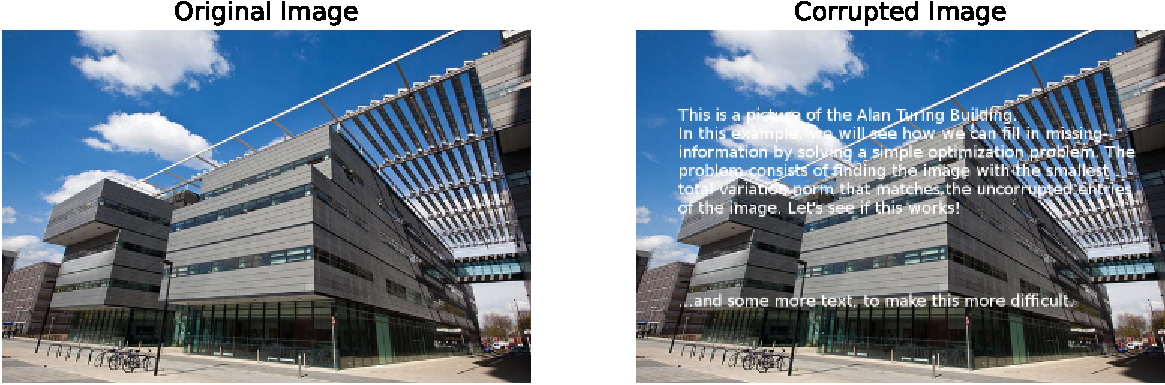
\includegraphics[width=1\textwidth]{images/alanturing1-crop.pdf}
\end{figure}

After having the images at our disposal, we determine which entries of the corrupted image are known. We store these in a {\em mask} $M$, with entries $m_{ijk}=1$ if the colour $k$ of the $(i,j)$-th pixel is known, and $0$ otherwise.

\begin{ipythonnb}[10]
# Each image is now an m x n x £\color{cogreen}3£ array, with each pixel 
# represented by three numbers between £\color{cogreen}0£ and £\color{cogreen}255£, 
# corresponding to red, green and blue
rows, cols, colours = U.shape

# Create a mask: this is a matrix with a £\color{cogreen}1£ if the corresponding 
# pixel is known, and zero else
M = np.zeros((rows, cols, colours))
for i in range(rows):
    for j in range(cols):
        for k in range(colours):
            if U[i, j, k] == Ucorr[i, j, k]:
                M[i, j, k] = 1
\end{ipythonnb}

We are now ready to solve the optimization problem using CVXPY. As the problem is rather big ($400\times 600\times 3 = 720000$ variables), it is important to choose a good solver that will solve the problem to sufficient accuracy in an acceptable amount of time. For the example at hand, we choose the SCS solver, which can be specified when calling the \textbf{solve} function.

\begin{ipythonnb}[11]
# Determine the variables and constraints
variables = []
constraints = []
for k in range(colours):
    X = Variable(rows, cols)
    # Add variables
    variables.append(X)
    # Add constraints by multiplying the relevant variable matrix 
    # elementwise with the mask
    constraints.append(mul_elemwise(M[:, :, k], X) == 
      \ (M[:, :, k], Ucorr[:, :, k]))

# Create a problem instance with
objective = Minimize(tv(variables[0],variables[1],variables[2]))

# Create a problem instance and solve it using the SCS solver
prob = Problem(objective, constraints)
prob.solve(verbose=True, solver=SCS)
\end{ipythonnb}
\begin{ipythonnbout}[11]
8263910.812250629
\end{ipythonnbout}

Now that we solved the optimization problem, we have a solution stored in 'variables'. We have to transform this back into an image and display the result.

\begin{ipythonnb}[12]
%matplotlib inline

# Load variable values into a single array.
Urec = np.zeros((rows, cols, colours), dtype=np.uint8)
for i in range(colours):
    Urec[:, :, i] = variables[i].value

fig, ax = plt.subplots(1, 2,figsize=(10, 5))

# Display the inpainted image.
ax[0].imshow(Urec);
ax[0].set_title("Inpainted Image")
ax[0].axis('off')

ax[1].imshow(np.abs(Ucorr[:,:,0:3] - Urec));
ax[1].set_title("Difference Image")
ax[1].axis('off');
\end{ipythonnb}

\begin{figure}[h!]
\centering
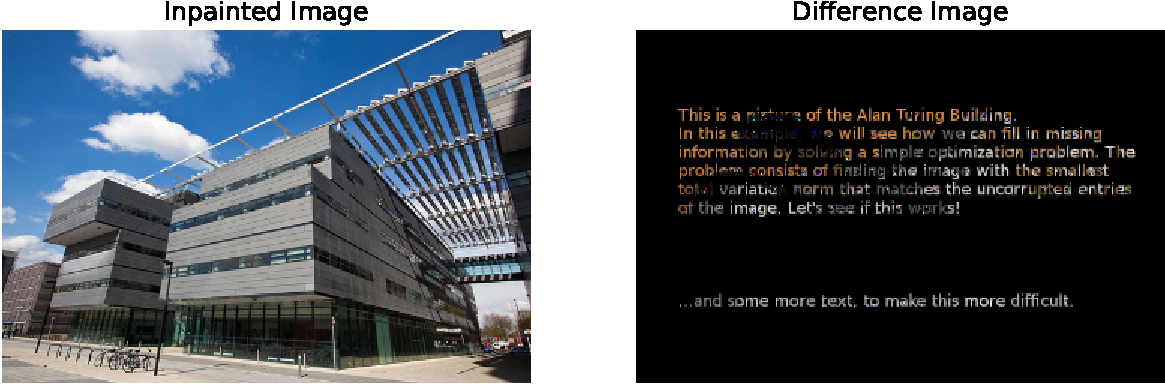
\includegraphics[width=1\textwidth]{images/alanturing2-crop.pdf}
\end{figure}

Another typical structure of images is that the \textbf{singular values} of the image, considered as matrix, decay quickly. The \textbf{singular value decomposition} (SVD) of a matrix $\mtx{A}\in \R^{m\times n}$ is the matrix product

\begin{equation*}
  \mtx{A} = \mtx{U}\mtx{\Sigma}\mtx{V}^{T},
\end{equation*}

where $\mtx{U}\in \R^{m\times m}$ and $\mtx{V}\in \R^{n\times n}$ are orthogonal matrices, and $\mtx{\Sigma}\in \R^{m\times n}$ is a diagonal matrix with entries $\sigma_{1},\dots,\sigma_{\mathrm{min}\{m,n\}}$ on the diagonal. Instead of minimizing the TV-norm of an image $\mtx{X}$, one may instead try to minimize the \textbf{Schatten 1-norm}, defined as the sum of the singular values, $\|\vct{U}\|_{S_1} = \sigma_1+\cdots+\sigma_{\mathrm{min}\{m,n\}}$. The problem is then

\begin{equation*}
  \minimize \|\vct{X}\|_{S_1} \subjto x_{ij} = u_{ij} \text{ for } (i,j) \in \Omega.
\end{equation*}

As we will see towards the end of the course, this is an instance of a type of convex optimization problem known as \textbf{semidefinite programming}. Luckily, CVXPY includes the Schatten 1-norm (also known as nuclear norm) as valid objective function, so we don't have to deal with the details of this problem. As the problem is computationally intensive, we just reproduce the result.

\begin{figure}[h!]
\centering
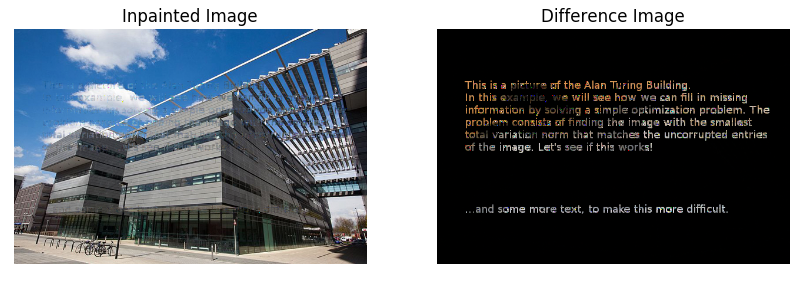
\includegraphics[width=1\textwidth]{images/nucnorm-inpaint.png}
\end{figure}

In this example, the result appears worse as in the problem involving the TV-norm. Alternatively, one may also use the $1$-norm of the image applied to a discrete cosine transfrom (DCT) or a discrete wavelet transform (DWT).

Of course, one could run the above examples for fun with different types of images in an attempt to get rid of certain parts. The image below show the result of applying the total variation inpainting procedure to set a parrot free.

\begin{figure}[h!]
\centering
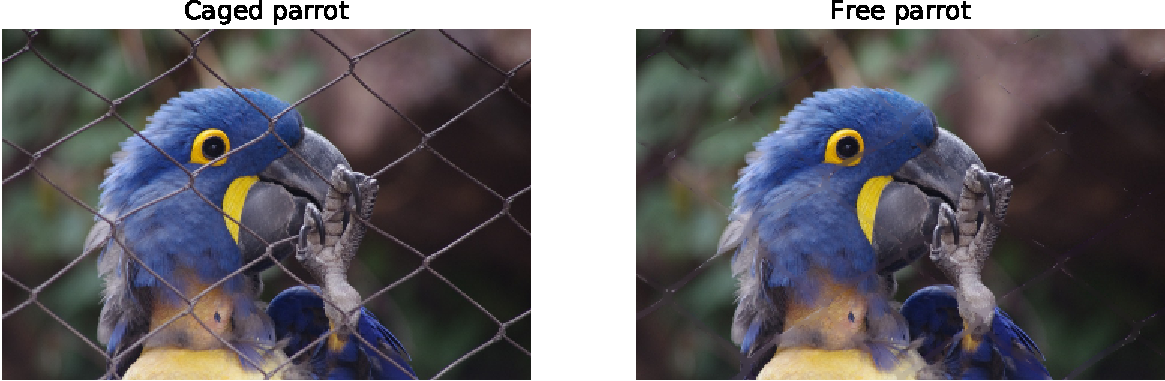
\includegraphics[width=1\textwidth]{images/parrot-crop.pdf}
\end{figure}
\end{example}


%-----------------------------------------------------------------------
% End of chap1.tex
%-----------------------------------------------------------------------

%%-----------------------------------------------------------------------
% Beginning of chap2.tex
%-----------------------------------------------------------------------
%
%  AMS-LaTeX sample file for a chapter of a monograph, to be used with
%  an AMS monograph document class.  This is a data file input by
%  chapter.tex.
%
%  Use this file as a model for a chapter; DO NOT START BY removing its
%  contents and filling in your own text.
% 
%%%%%%%%%%%%%%%%%%%%%%%%%%%%%%%%%%%%%%%%%%%%%%%%%%%%%%%%%%%%%%%%%%%%%%%%


\chapter*{Lecture 2}
\addcontentsline{toc}{chapter}{Lecture 2}
\addtocounter{chapter}{2}
%\numberwithin{section}{chapter}
\numberwithin{equation}{chapter}
\numberwithin{theorem}{chapter}


In this lecture we will study the unconstrained problem
\begin{equation}\label{eq:uncont}
 \minimize f(\vct{x}),
\end{equation}
where $\vct{x}\in \R^n$. Optimality conditions aim to identify properties that potential minimizers need to satisfy in relation to $f(\vct{x})$. We will review the well known local optimality conditions for differentiable functions from calculus. We then introduce convex functions and discuss some of their properties.

\section{Unconstrained optimization}
Solutions to~\eqref{eq:uncont} come in different flavours, as in the following definition.

\begin{definition}
A point $\vct{x}^*\in \R^n$ is a
\begin{itemize}
 \item  {\em global minimizer} of~\eqref{eq:uncont} if for all $\vct{x}\in U$, $f(\vct{x}^*)\leq f(\vct{x})$;
 \item a {\em local minimizer}, if there is an open neighbourhood $U$ of $\vct{x}$ such that $f(\vct{x}^*)\leq f(\vct{x})$ for all $\vct{x}\in U$;
 \item a {\em strict local minimizer}, if there is an open neighbourhood $U$ of $\vct{x}$ such that $f(\vct{x}^*)<f(\vct{x})$ for all $\vct{x}\in U$;
 \item an {\em isolated minimizer} if there is an open neighbourhood $U$ of $\vct{x}^*$ such that $\vct{x}^*$ is the only local minimizer in $U$.
 \end{itemize}
\end{definition}

Without any further assumptions on $f$, finding a minimizer is a hopeless task: we simply can't examine the function at {\em all} points in $\R^n$. 
The situation becomes more tractable if we assume some {\em smoothness} conditions. Recall that $C^k(U)$ denotes the set of functions that are $k$ times continuously differentiable on some set $U$. The following {\em first-order} necessary condition for optimality is well known. We write $\nabla f(\vct{x})$ for the gradient of $f$ at $\vct{x}$, i.e., the vector 
\begin{equation*}
 \nabla f(\vct{x}) = \left(\frac{\partial f}{\partial x_1}(\vct{x}),\dots,\frac{\partial f}{\partial x_n}(\vct{x})\right)^{\trans}
\end{equation*}


\begin{theorem}
 Let $\vct{x}^*$ be a local minimizer of $f$ and assume that $f\in C^1(U)$ for a neighbourhood of $U$ of $\vct{x}^*$. Then $\nabla f(\vct{x}^*) = \zerovct$. 
\end{theorem}

There are simple examples that show that this is not a sufficient condition: maxima and saddle points will also have a vanishing gradient. If we have access to {\em second-order information}, in form of the second derivative, or Hessian, of $f$, then we can say more. Recall that the Hessian of $f$ at $\vct{x}$, $\nabla^2f(\vct{x})$, is the $d\times d$ symmetric matrix given by the second derivatives,
\begin{equation*}
 \nabla^2f(\vct{x}) = \left(\frac{\partial^2 f}{\partial x_i \partial x_j}\right)_{1\leq i,j\leq n}.
\end{equation*}
In the one-variable case we have learned that if $x^*$ is a local minimizer of $f\in C^2([a,b])$, then $f'(x^*)=0$ {\em and} $f''(x^*)\geq 0$. Moreover, the conditions $f'(x^*)=0$ {\em and} $f''(x^*)>0$ guarantee that we have a local minimizer. These conditions generalise to higher dimension, but first we need to know what $f''(x)>0$ when we have more than one variable.

Recall also that a matrix $\mtx{A}$ is \textbf{positive semidefinite}, written $\mtx{A}\succeq \zerovct$, if for every $\vct{x}\in \R^d$, $\vct{x}^{\top}\mtx{A}\vct{x}\geq 0$, and positive definite, written $\mtx{A}\succ \zerovct$, if $\vct{x}^{\top}\mtx{A}\vct{x}>0$. The property that the Hessian matrix is positive semidefinite is a multivariate generalization of the property that the second derivative is nonnegative. The known conditions for a minimizer involving the second derivative generalize accordingly.

\begin{theorem}
 Let $f\in C^2(U)$ for some open set $U$ and $\vct{x}^*\in U$. 
 If $\vct{x}^*$ is a local minimizer, then $\nabla f(\vct{x}^*)=0$ and $\nabla^2f(\vct{x}^*)$  is positive semidefinite. Conversely, if $\nabla f(\vct{x}^*)=\zerovct$ and $\nabla^2f(\vct{x}^*)$ is positive definite, then $\vct{x}^*$ is a strict local minimizer. 
\end{theorem}

Unfortunately, the above criteria are not able to identify global minimizers, as differentiability is a local property.

\section{Convex functions} We now come to the central notion of this course.  

\begin{definition} A set $C\subseteq \R^n$ is \textbf{convex} if for all $\vct{x},\vct{y}\in C$ and $\lambda \in [0,1]$, the line $\lambda \vct{x}+(1-\lambda)\vct{y}\in C$. A \textbf{convex body} is a convex set that is closed and bounded.
\end{definition}

\begin{definition}
Let $S\subseteq \R^n$. 
A function $f\colon S\to \R$ is called {\em convex} if $S$ is convex and for all $\vct{x},\vct{y}\in S$ and $\lambda\in [0,1]$,
\begin{equation*}
 f(\lambda \vct{x}+(1-\lambda)\vct{y})\leq \lambda f(\vct{x})+(1-\lambda)f(\vct{y}).
\end{equation*}
The function $f$ is called {\em strictly convex} if
\begin{equation*}
 f(\lambda \vct{x}+(1-\lambda)\vct{y})< \lambda f(\vct{x})+(1-\lambda)f(\vct{y}).
\end{equation*}
A function $f$ is called {\em concave}, if $-f$ is convex. 
\end{definition}

Figure~\ref{fig:convfun} illustrates how a convex function of one variable looks like. The graph of the function lies below any line connecting two points on it.

\begin{figure}[h!]
\centering
 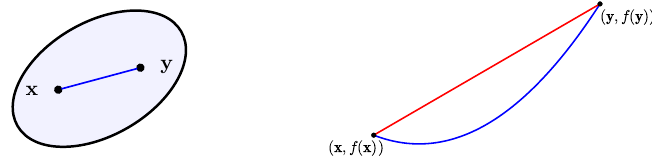
\includegraphics[width=0.8\textwidth]{images/convset.png}
 \caption{A convex set and a convex function}\label{fig:convfun}
\end{figure}

Convex function have pleasant properties, while at the same time covering many of the functions that arise in applications. Perhaps the most important property is that local minima are global minima.

\begin{theorem}
 Let $f\colon \R^n\to \R$ be a convex function. Then any local minimizer of $f$ is a global minimizer.
\end{theorem}

\begin{proof}
 Let $\vct{x}^*$ be a local minimizer and assume that it is not a global minimizer. Then there exists a vector $\vct{y}\in \R^d$ such that $f(\vct{y})<f(\vct{x}^*)$. Since $f$ is convex, for any $\lambda\in [0,1]$ and $\vct{x}=\lambda \vct{y}+(1-\lambda)\vct{x}^*$ we have
 \begin{equation*}
  f(\vct{x}) \leq \lambda f(\vct{y})+(1-\lambda) f(\vct{x}^*) < \lambda f(\vct{x}^*)+(1-\lambda)f(\vct{x}^*) = f(\vct{x}^*).
 \end{equation*}
This holds for all $\vct{x}$ on the line segment connecting $\vct{y}$ and $\vct{x}^*$. Since every open neighbourhood $U$ of $\vct{x}^*$ contains a bit of this line segment, this means that every open neighbourhood $U$ of $\vct{x}^*$ contains an $\vct{x}\neq \vct{x}^*$ such that $f(\vct{x})\leq f(\vct{x}^*)$, in contradiction to the assumption that $\vct{x}^*$ is a local minimizer. It follows that $\vct{x}^*$ has to be a global minimizer.
\end{proof}

\begin{remark} Note that in the above theorem we made no assumptions about the differentiability of the function $f$! In fact, while a convex function is always {\em continuous}, it need not be differentiable. The function $f(x) = |x|$ is a typical example: it is convex, but not differentiable at $x=0$.
\end{remark}

\begin{example}
 Affine functions $f(\vct{x})=\ip{\vct{x}}{\vct{a}}+b$ and the exponential function $e^x$ are examples of convex functions. 
\end{example}

\begin{example}
 In optimization we will often work with functions of matrices, where an $m\times n$ matrix is considered as a vector in $\R^{m\times n}\cong \R^{mn}$. If the matrix is symmetric, that is, if $\mtx{A}^{\trans}=\mtx{A}$, then we only care about the upper diagonal entries, and we consider the space $\mathcal{S}^n$ of symmetric matrices as a vector space of dimension $n(n+1)/2$ (the number of entries on and above the main diagonal). Important functions on symmetric matrices that are convex are the operator norm $\norm{\mtx{A}}_2$, defined as
 \begin{equation*}
  \norm{\mtx{A}}_2 := \max_{\vct{x}\colon \norm{\vct{x}}\leq 1} \frac{\norm{\mtx{A}\vct{x}}_2}{\norm{\vct{x}}_2},
 \end{equation*}
or the function $\log \det(\mtx{X})$, defined on the set of {\em positive semidefinite} symmetric matrices $\mathcal{S}_+^n$.
\end{example}

There are useful ways of characterising convexity using differentiability.
\begin{theorem}
\begin{enumerate}
 \item Let $f\in C^1(\R^n)$. Then $f$ is convex if and only if for all $\vct{x}, \vct{y}\in \R^n$,
 \begin{equation*}
  f(\vct{y})\geq f(\vct{x})+\nabla f(\vct{x})^{\trans} (\vct{y}-\vct{x}).
 \end{equation*}
 \item Let $f\in C^2(\R^n)$. Then $f$ is convex if and only if $\nabla^2 f(\vct{x})$ is positive semidefinite. If $\nabla^2f(\vct{x})$ is positive definite, then $f$ is strictly convex.
 \end{enumerate}
\end{theorem}

\begin{example}\label{ex:quad}
 Consider a quadratic function of the form
 
 \begin{equation*}
f(\vct{x}) = \frac{1}{2}\vct{x}^{\trans}\mtx{A}\vct{x}+\vct{b}^{\trans}\vct{x}+c, 
 \end{equation*}
 
 where $\mtx{A}\in \R^{n\times n}$ is symmetric. Writing out the product, we get
 
 \begin{align*}
   \mtx{x}^{T}\mtx{A}\vct{x} &= \begin{pmatrix} x_1 & \cdots & x_n
   \end{pmatrix}
   \begin{pmatrix}
   a_{11} & \cdots & a_{1n}\\
   \vdots & \ddots & \vdots\\
   a_{n1} & \cdots & a_{nn}
   \end{pmatrix}
   \begin{pmatrix}
   x_1\\ \vdots \\ x_n
   \end{pmatrix} \\
   &= \begin{pmatrix}
   x_1 & \cdots & x_n
   \end{pmatrix}
   \begin{pmatrix}
   a_{11}x_1+\cdots+a_{1n}x_n\\
   \vdots \\
   a_{n1}x_1+\cdots+a_{nn}x_n
   \end{pmatrix} = \sum_{i=1}^n \sum_{j=1}^n a_{ij} x_i x_j.
 \end{align*} 
 
 Because $\mtx{A}$ is symmetric, we have $a_{ij}=a_{ji}$, and the above product simplifies to
 
 \begin{equation*}
 \vct{x}^{T}\mtx{A}\vct{x} = \sum_{i=1}^n a_{ii} x_i^2 + 2\sum_{1\leq i<j\leq n} a_{ij}x_i x_j.
 \end{equation*}
 
 This is a quadratic function, because it involves products of the $x_i$. The gradient and the Hessian of $f(\vct{x})$ are found by computing the partial derivatives of $f$:
 
 \begin{equation*}
 \frac{\partial f}{\partial x_i} = \sum_{j=1}^n a_{ij} x_j + b_i, \quad \frac{\partial^2 f}{\partial x_i \partial x_j} = a_{ij}.
 \end{equation*}
 
 In summary, we have
 \begin{equation*}
   \nabla f(\vct{x}) = \mtx{A}\vct{x} + \vct{b}, \quad \nabla^2f(\vct{x}) = \mtx{A}.
 \end{equation*}
 
 Using the previous theorem, we see that $f$ is convex \textbf{if and only if} $\mtx{A}$ is positive semidefinite. A typical example for such a function is
 
 \begin{equation*}
   f(\vct{x}) = \|\mtx{A}\vct{x}-\vct{b}\|^2 = (\mtx{A}\vct{x}-\vct{b})^{T}(\mtx{A}\vct{x}-\vct{b}) = \vct{x}^{T}\mtx{A}^{T}\mtx{A}\vct{x} -2\vct{b}^{T}\mtx{A}\vct{x}+\vct{b}^T\vct{b}.
 \end{equation*}
 
 The matrix $\mtx{A}^T\mtx{A}$ is always symmetric and positive semidefinite (why?) so that the function $f$ is convex.
\end{example}

A convenient way to visualise a function $f\colon \R^2\to \R$ is through \textbf{contour plots}. A \textbf{level set} of the function $f$ is a set of the form
\begin{equation*}
  \{\vct{x}\mid f(\vct{x}) = c\},
\end{equation*}

where $c$ is the \textbf{level}. Each such level set is a curve in $\R^2$, and a contour plot is a plot of a collection of such curves for various $c$. If one colours the areas between adjacent curves, one gets a plot as in the following figure. A {\em convex function} is has the property that there is only one {\em sink} in the contour plot.

\begin{ipythonnb}
\\# import numpy as np
import numpy.linalg as la
import matplotlib.pyplot as plt
% matplotlib inline

# Create random data: we use the randn function
X = np.random.randn(3,2)
y = np.random.randn(3)

# Solve least squares problem minimize \|X\beta-y\|^2
# the index 0 says that we get the first component of the solution
# (the function lstsq give more output than just the beta vector)
beta = la.lstsq(X,y)[0]

# Create function and plot the contours
def f(a,b):
    return sum((a*X[:,0]+b*X[:,1]-y)**2)

# Find the "right" boundaries around the minimum
xx = np.linspace(beta[0]-8,beta[0]+8,100)
yy = np.linspace(beta[1]-8,beta[1]+8,100)
XX, YY = np.meshgrid(xx,yy)

Z = np.zeros(XX.shape)
for i in range(Z.shape[0]):
    for j in range(Z.shape[1]):
        Z[i,j] = f(XX[i,j],YY[i,j])

cmap = plt.cm.get_cmap("coolwarm")
plt.contourf(XX,YY,Z, cmap = cmap)
plt.show()
\end{ipythonnb}

\begin{figure}[h!]
\centering
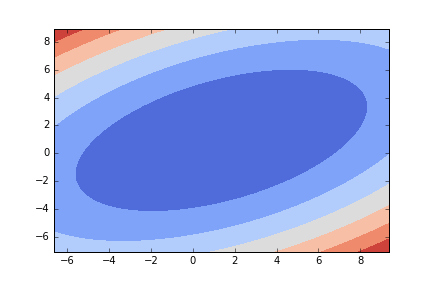
\includegraphics[width=0.6\textwidth]{images/contourplot.png}
\end{figure}


%-----------------------------------------------------------------------
% End of chap1.tex
%-----------------------------------------------------------------------


%\appendix
%\include{appendix1}

%\backmatter
%\include{biblio}
%\include{index}
\end{document}

%-----------------------------------------------------------------------
% End of chapter.tex
%-----------------------------------------------------------------------
